\section{Wetter und Klima}
\begin{frame}
	% TODO: Wetter vs. Klimadaten Dortmund: zB Osterwetter vs klassisches Niederschlags-Temperatur-Diagramm anfertigen

	% TODO: Daten dazu beim dwd oder bei der Stadt Dortmund Stichwort Opendata -Weather bzw. Witterung

	%TODO: Campuswetter der TU NICHT nutzbar, da urheberrechtlich geschützt
	\frametitle{Wetter und Klima}
	\begin{columns}[onlytextwidth]
		\begin{column}[t]{0.49\linewidth}
			\textbf{Wetter}\\
			\textit{\enquote{ist der physikalische Zustand der Atmosphäre an einem bestimmten Ort zu einem \alert{bestimmten Zeitpunkt} oder in einem kurzen Zeitraum.}}
			\begin{itemize}
				\item Gekennzeichnet durch Ist-Werte von Temperatur, Luftfeuchtigkeit, Niederschlag, ...
				\item Ist was wir täglich mit unseren Sinnen erleben
			\end{itemize}
		\end{column}%
		\begin{column}[t]{0.49\linewidth}
			\textbf{Klima}\\
			\textit{\enquote{ist der mittlere Zustand der Atmosphäre an einem bestimmten Ort über einen \alert{längeren Zeitraum.}}}
			\begin{itemize}
				\item Gekennzeichnet durch statistische Mittelwerte (circa 30 Jahre) der selben Größen
				\item Ist entscheidend für die Entwicklung der Ökosysteme
			\end{itemize}
		\end{column}%
	\end{columns}
	\pause
	\bigskip
	\begin{center}
		Das (durchschnittliche) Wetter macht das Klima, \\
		das Klima bestimmt das (wahrscheinliche) Wetter.
	\end{center}

	\vfill
	\tiny{Zitate von \url{https://www.umweltbundesamt.de/service/uba-fragen/was-ist-eigentlich-klima}}

	\note{
	Klima
	\begin{itemize}
		\item Auch definiert als Zustand des klimatischen Systems, Weltorganisation für Meterologie (WMO)
		\item Betrachtung verschiedener Parameter wie Temperatur, Niederschlag, Windgeschwindigkeiten (WMO)
		\item Betrachtet werden u.a. Mittelwert, Abweichung und Wahrscheinlichkeit des Auftretens extremer Ereignisse z.B. Dürren %M.Latif, Klimawandel und Klimadynamik S. 11
		\item Aus dem Griechischen: \textit{klinein} $\equiv$ neigen $\rightarrow$ Neigung der Erdachse
	\end{itemize}
	}

\end{frame}

\begin{frame}
	\frametitle{Klima - Neigung der Erdachse}
	\begin{figure}
		\centering
		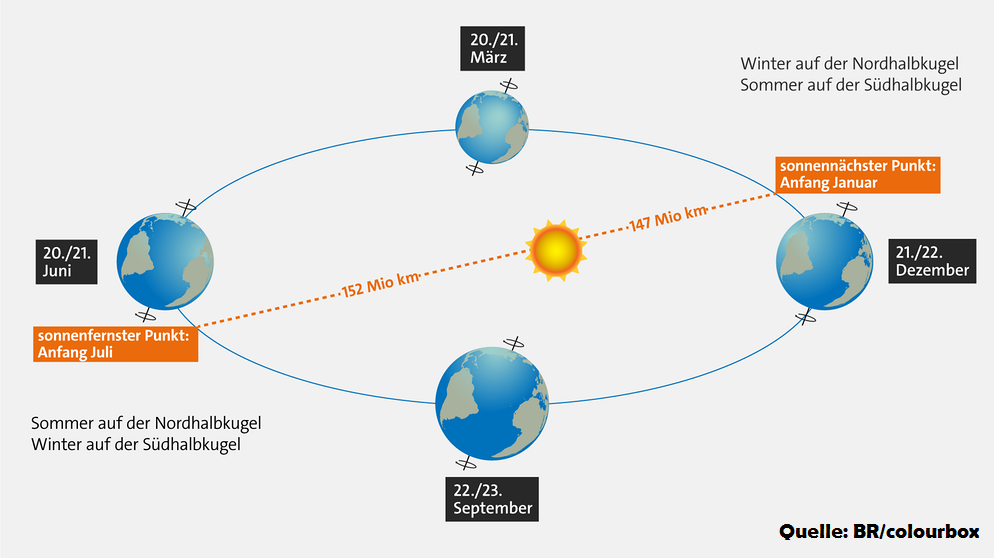
\includegraphics[width=0.5\linewidth]{bilder/Erdumlaufbahn_DWD.png}
		\caption{Neigung der Erdachse als Ursache für die Jahreszeiten, Quelle: Deutscher Wetterdienst}
	\end{figure}

	\begin{itemize}
		\item Die Neigung der Erde ist entscheidend für die Sonneneinstrahlung auf der Erde
		\item [$\rightarrow$] und damit verantwortlich für die Jahreszeiten und das Klima auf der Nord und Südhalbkugel
	\end{itemize}

	\note{
	\begin{itemize}
		\item[] Erde rotiert um die Sonne und um die eigene Achse
		\item[]	Neigung der Erdachse momentan etwa \SI{23,5}{°}
		\item[$\rightarrow$] Jahreszeiten
	\end{itemize}
	}
\end{frame}

\begin{frame}
\frametitle{Klima - Eiszeitzyklen}
\begin{figure}
	\centering
	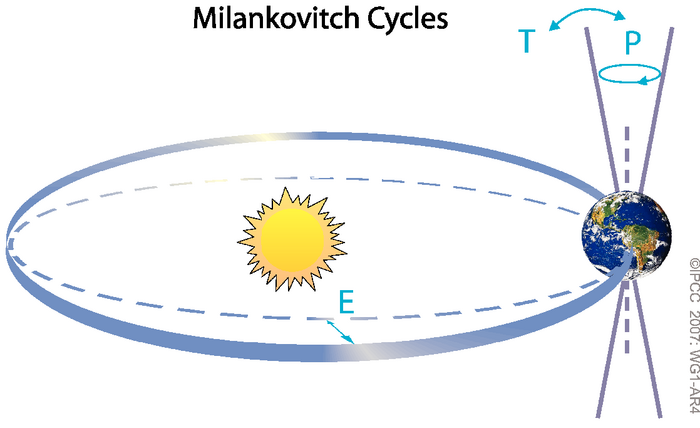
\includegraphics{bilder/milankovitch_IPCC2007_AR4.png}
	\caption{Milankovitch-Zyklen: Periodische Änderungen der Erdbahnparameter, Quelle: IPCC 2007, WG1, Kapitel 6}
\end{figure}
\begin{itemize}
	\item[E] Veränderung der Ausdehnungsrichtung der Erdbahn (Exzentrizität)% - aktuell: 0,017 perfekter Kreis bei 0, leicht elliptisch bei 0,05
	\item[T] Veränderung des Neigungswinkels der Erdachse (eng. tilt)
	\item[P] Schwankung der Erde um die Erdachse (Präzession) % da die Erde keine perfekte Kugel ist
	\item[$\rightarrow$] verursachen Eiszeitzyklen, sowie deren Warm- und Kaltphasen
	\item[$\rightarrow$] langfristiger Einfluss auf das Klima
\end{itemize}

\note{
\begin{itemize}
	\item[] Milankovic in den 1930er Jahren, Eiszeitzyklen
	\item[] Exzentrizität: Erdbahn variiert
	\begin{itemize}
		\item[] Periode: etwa 1 mio. Jahre, variiert zwischen \num{0,002} und \num{0,05}
		\item[] Momentan: \num{0,017}, perfekter Kreis bei 0, leicht elliptisch bei \num{0,05}.
		\item[] Ursache: Störung durch die anderen Planeten des Sonnensystems, im wesentlichen Jupiter und Saturn.
		\item[] Folge: Solare Einstrahlung wird um weniger als \SI{1}{W\per m} geändert.
	\end{itemize}
	\item[] Neigung der Erdachse
	\begin{itemize}
		\item[] Periode: \num{41000} Jahre, Auslenkung zwischen \SIrange{22}{24,5}{°}
		\item[] Momentan: \SI{23,5}{°}
		\item[] Ursache: Gravitationseinfluss der anderen Himmelskörper im Sonnensystem
		\item[] Folge: Verstärkt oder schwächt jahreszeitliche Unterschiede.
		\item[] Keine Veränderung der gemittelten, jährlichen Sonneneinstrahlung.
	\end{itemize}
	\item[] Präzession der Erde, taumeln um die eigene Achse
	\begin{itemize}
		\item[] Periode: etwa \num{20000} Jahre
		\item[] Ursache: Die Erde ist keine perfekte Kugel.
		\item[] Folge: Jahreszeiten treten nicht immer im gleichen Bahnpunkt der Erdbahnellipse auf.
	\end{itemize}
\end{itemize}
}
\end{frame}


\begin{frame}
	\frametitle{Klimaänderung}
	\begin{block}{Klimaänderung}
		Erkennbare (messbare) Änderung Klimas über einen gewissen Zeitraum (z.B. 30 Jahre) %M.Latif Klimawandel und Klimadynamik S. 13
		Spürbar durch Änderung atmosphärischer Größen wie der Temperatur
	\end{block}

	\uncover<2->{
	\begin{figure}
		\centering
		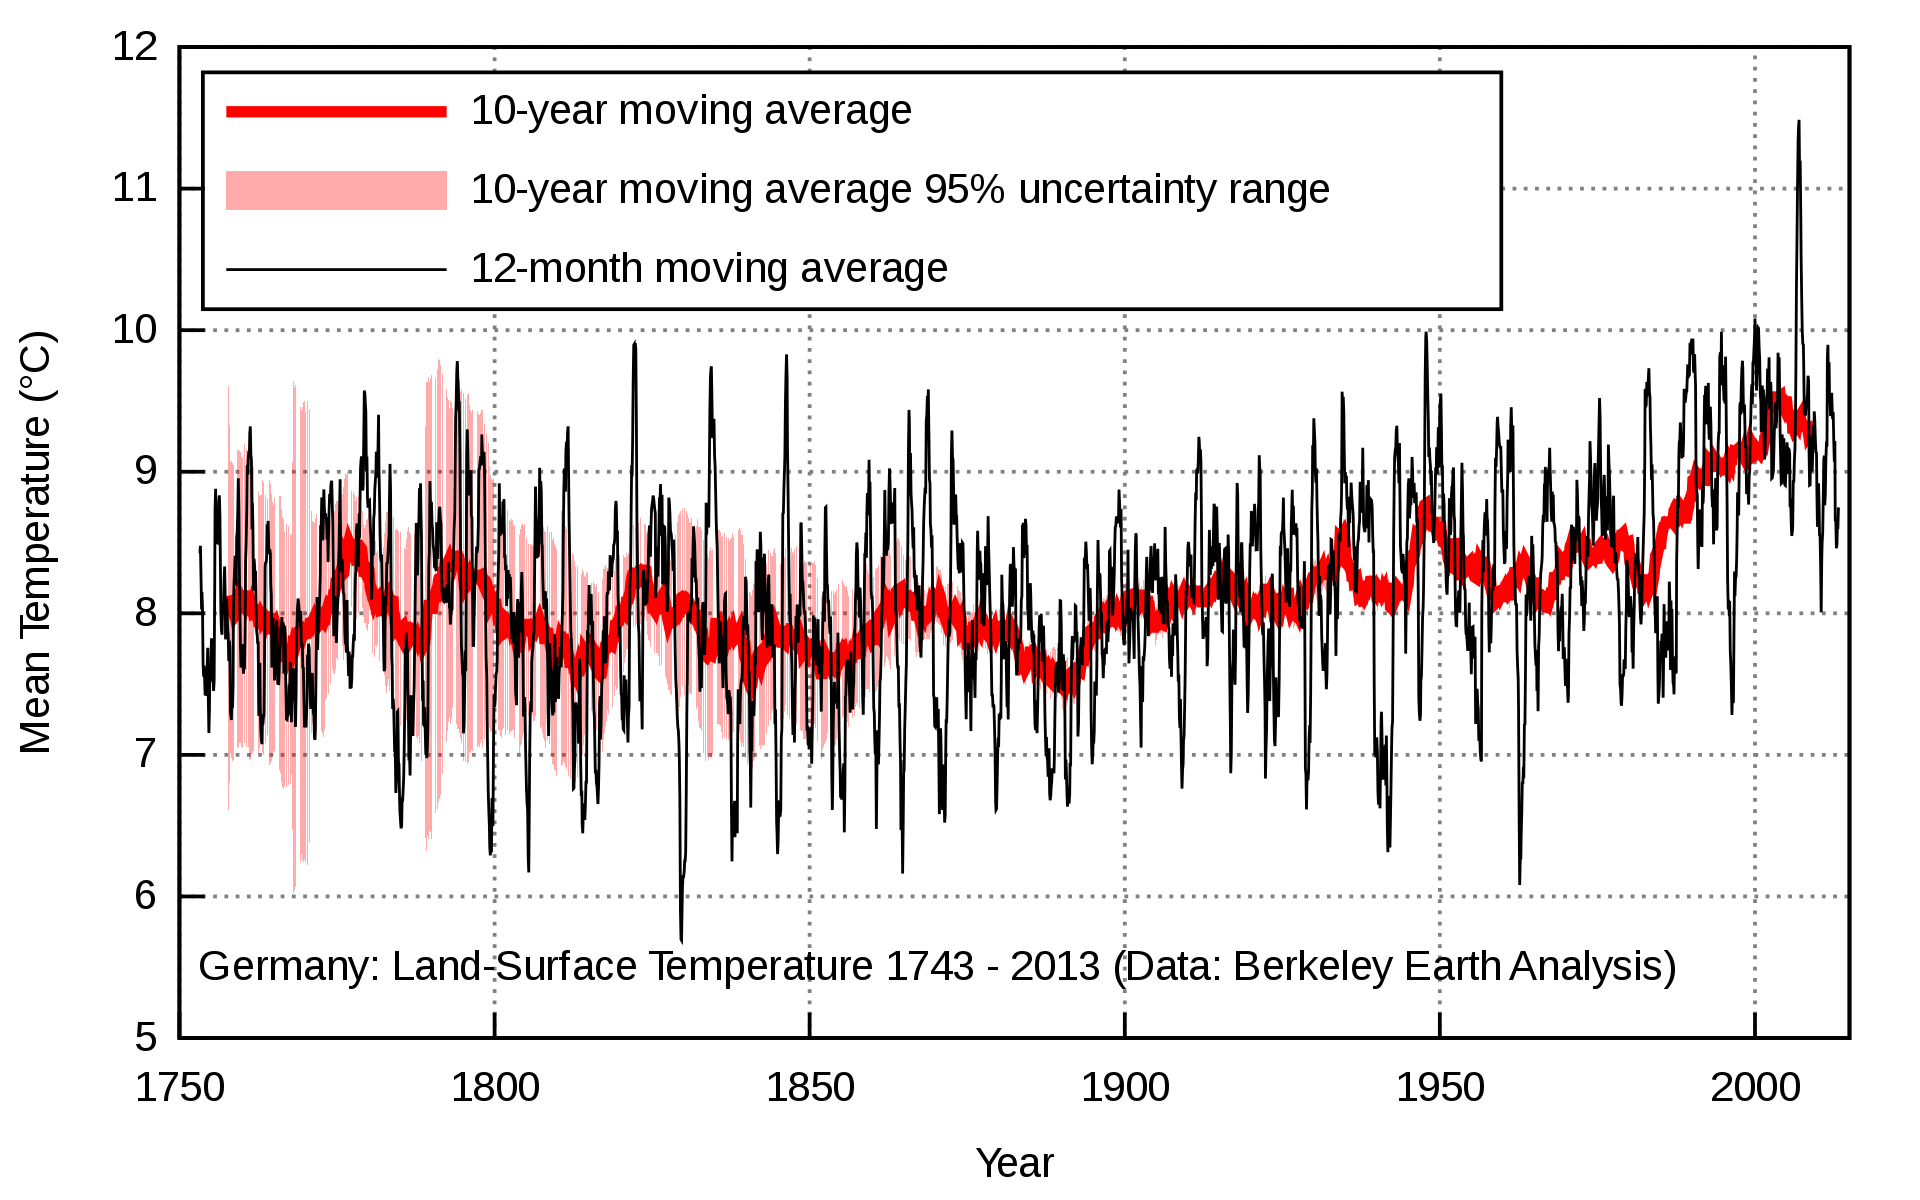
\includegraphics[width=0.6\linewidth]{bilder/Temp_Deutschland_1743-2013_Berkley_Wiki.png}
		\caption{Entwicklung der mittleren Jahrestemperaturen in Deutschland, Quelle: Wikipedia, Daten: Berkeley Earth Surface Temperature Project}
	\end{figure}
	}

	%TODO Bild mit 30 Jahre moving average erstellen
	\note{
	\begin{itemize}
		\item[] mittlere Temperaturen in Deutschland pro Jahr von 1743 bis 2013
		\item[] 10 Jahre moving average, Fluktuation, aber Temperaturanstieg
		\item[] 30 Jahre moving average, weniger Schwankungen, kleiner, aber deutlicher Temperaturanstieg
	\end{itemize}
	}

\end{frame}

\begin{frame}
	\frametitle{Klimavorhersagen} %TODO
	\begin{itemize}
		\item Die statistischen Eigenschaften des Wetters lassen sich längerfristig Vorhersagen.
		\item[$\rightarrow$] Jahreszeiten, Monsunregen, etc.. %TODO: Bedingungen dafür in  Kapitel 3.3 aus M.Latif nachlesen
		\item Atmosphärische Änderungen im Kontext des Erdsystems
		\item [$\rightarrow$] Hydrosphäre, Kryosphäre, Biospähre, Pedosphäre und Lithosphäre % Stichwort Wechselwirkungen
	\end{itemize}

	\note{
	\begin{itemize}
		\item[] Kapitel 3.3 M. Latif
	\end{itemize}
	}
\end{frame}
